\documentclass[12pt]{exam}
\usepackage{libertine}
\usepackage[utf8]{inputenc}
\usepackage[margin=1in]{geometry}
\usepackage{amsmath,amssymb,amsthm}
\usepackage{multicol}
\usepackage[shortlabels]{enumitem}
\usepackage{siunitx}
\usepackage{cancel}
\usepackage{graphicx}
\usepackage{pgfplots}
\usepackage{listings}
\usepackage{tikz}
\usepackage{booktabs}
\usepackage{indentfirst}


\pgfplotsset{width=10cm,compat=1.9}
\usepgfplotslibrary{external}
% Uncomment if your compiler has shell-escape enabled:
% \tikzexternalize

\newcommand{\class}{Research in CompMath} 
\newcommand{\examnum}{Homework 1} 
\newcommand{\examdate}{9/3/2026}

\begin{document}
\pagestyle{plain}
\thispagestyle{empty}

\noindent
\begin{tabular*}{\textwidth}{l @{\extracolsep{\fill}} r @{\extracolsep{6pt}} l}
\textbf{\class} & \textbf{Name:} & \textit{Mary Kim}\\ 
\textbf{\examdate} &&\\
\end{tabular*}\\
\rule[2ex]{\textwidth}{2pt}
% -------

1.4 Exercises 1, 8, 14
\begin{enumerate}[listparindent=1.5em]

\item Let $A = \{1, 3, 12, 35\}$, $B = \{3, 7, 12, 20\}$, and $C = \{x \mid x \text{ is a prime number}\}$. List the elements of the following sets. Are any of the sets below disjoint from any of the others? Are any of the sets below subsets of any others?

(a) $A \cap B = \{3, 12\}$

(b) $(A \cup B) \setminus C = \{1, 12, 20, 35\}$

(c) $A \cup (B \setminus C) = \{1, 3, 12, 20, 35\}$

$A \cap B$ and $(A \cup B) \setminus C$ are subsets of $A \lor (B \setminus C)$.

\item Use any method you wish to verify the following identities:

(a) $(A \setminus B) \cap C = (A \cap C) \setminus B$.
\\ $x \in (A \setminus B) \cap C \rightarrow (x \in A \land \lnot (x \in B)) \land (x \in C) = (x \in A) \land \lnot (x \in B) \land (x \in C)$
\\ $x \in (A \cap C) \setminus B \rightarrow (x \in A \land x \in C) \land \lnot (x \in B) = (x \in A) \land (x \in C) \land \lnot (x \in B)$
\\ By commutative property, the above expressions are equal to each other. 

(b) $(A \cap B) \setminus B = \emptyset$.
\\ $(x \in A) \land (x \in B) \land \lnot (x \in B)$
\\ This statement contradicts itself since $x$ cannot be in $B$ and not in $B$ at the same time, so therefore the left hand side of the statement does not hold true and therefore it must be that there are no data values in the set. 

(c) $A \setminus (A \setminus B) = A \cap B$.

\item Use Venn diagrams to show that the associative law holds for symmetric difference; that is, for any sets $A$, $B$, and $C$, $A \Delta (B \Delta C) = (A \Delta B) \Delta C$.

\subsubsection*{Venn Diagram Illustration}

Both of the Venn Diagrams for $A \Delta (B \Delta C)$ and  $(A \Delta B) \Delta C$ are the same, as seen below. 

\begin{center}
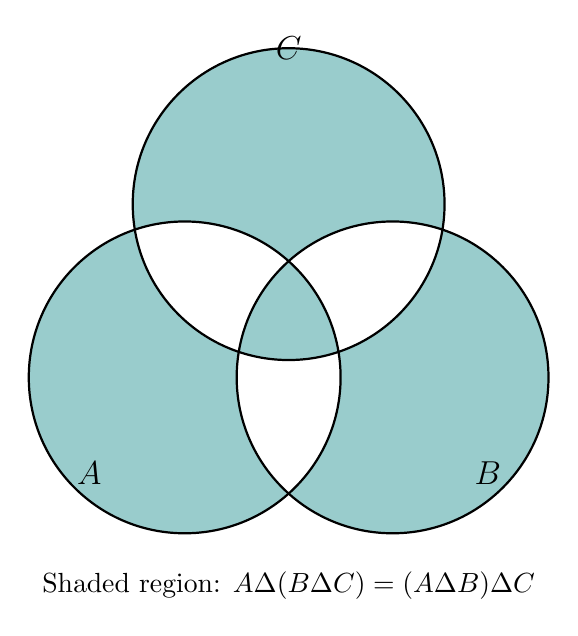
\begin{tikzpicture}[scale=1.1]
    \coordinate (A) at (0, 0);
    \coordinate (B) at (2.4, 0);
    \coordinate (C) at (1.2, 2.0);
    \def\R{1.8cm}

    % 1. Only A: A \ (B U C)
    \begin{scope}
        \clip (A) circle (\R);
        \fill[teal!40] (-3,-3) rectangle (5,5);
    \end{scope}
    \begin{scope}
        \clip (A) circle (\R);
        \clip (B) circle (\R);
        \fill[white] (-3,-3) rectangle (5,5);
    \end{scope}
    \begin{scope}
        \clip (A) circle (\R);
        \clip (C) circle (\R);
        \fill[white] (-3,-3) rectangle (5,5);
    \end{scope}

    % 2. Only B: B \ (A U C)
    \begin{scope}
        \clip (B) circle (\R);
        \fill[teal!40] (-3,-3) rectangle (5,5);
    \end{scope}
    \begin{scope}
        \clip (B) circle (\R);
        \clip (A) circle (\R);
        \fill[white] (-3,-3) rectangle (5,5);
    \end{scope}
    \begin{scope}
        \clip (B) circle (\R);
        \clip (C) circle (\R);
        \fill[white] (-3,-3) rectangle (5,5);
    \end{scope}

    % 3. Only C: C \ (A U B)
    \begin{scope}
        \clip (C) circle (\R);
        \fill[teal!40] (-3,-3) rectangle (5,5);
    \end{scope}
    \begin{scope}
        \clip (C) circle (\R);
        \clip (A) circle (\R);
        \fill[white] (-3,-3) rectangle (5,5);
    \end{scope}
    \begin{scope}
        \clip (C) circle (\R);
        \clip (B) circle (\R);
        \fill[white] (-3,-3) rectangle (5,5);
    \end{scope}

    % 4. Intersection of all three: A \cap B \cap C
    \begin{scope}
        \clip (A) circle (\R);
        \clip (B) circle (\R);
        \clip (C) circle (\R);
        \fill[teal!40] (-3,-3) rectangle (5,5);
    \end{scope}

    % Outlines and Labels
    \draw[thick] (A) circle (\R);
    \draw[thick] (B) circle (\R);
    \draw[thick] (C) circle (\R);

    \node at (-1.1, -1.1) {\large $A$};
    \node at (3.5, -1.1) {\large $B$};
    \node at (1.2, 3.8) {\large $C$};

    \node at (1.2, -2.4) {Shaded region: $A \Delta (B \Delta C) = (A \Delta B) \Delta C$};
\end{tikzpicture}
\end{center}

\end{enumerate}

\vspace{1em}
1.5 Exercises 2, 8, 12
\begin{enumerate} 

    \item Analyze the logical forms of the following statements:
    
(a) Mary will sell her house only if she can get a good price and find a
nice apartment.
\\S: Mary will sell her house.
\\P: She gets a good price.
\\A: She finds a nice apartment. 
\\This is represented by the logical statement: 
\\  S $\rightarrow (P \land A)$

(b) Having both a good credit history and an adequate down payment is a
necessary condition for getting a mortgage.
\\M: Someone gets a mortgage.
\\C: Someone has a good credit history.
\\D: Someone has an adequate down payment.
\\This is represented by the logical statment: 
\\ M $\rightarrow (C \land D)$

(c) John will drop out of school, unless someone stops him. (Hint: First
try to rephrase this using the words if and then instead of unless.)
\\If someone does not stop John, he will drop out of school.
\\J: John will drop out of school.
\\S: Someone stops him. 
\\ $\lnot S \rightarrow J$

(d) If x is divisible by either 4 or 6, then it isn’t prime.
\\F: X is divisible by 4 
\\S: X is divisible by 6
\\P: X is prime
\\ $(F \lor S) \rightarrow \lnot P$

\item 8. 
\\(a) Show that $(P \rightarrow Q) \land (Q \rightarrow R)$ is equivalent to $(P \rightarrow R) \land [(P \leftrightarrow Q) \lor (R \leftrightarrow Q)$].

\begin{table}[htbp]
\centering
\resizebox{\textwidth}{!}{%
\begin{tabular}{ccccccccccc}
\toprule
$P$ & $Q$ & $R$ & $P \to Q$ & $Q \to R$ & $(P \to Q) \land (Q \to R)$ & $P \to R$ & $P \leftrightarrow Q$ & $R \leftrightarrow Q$ & $(P \leftrightarrow Q) \lor (R \leftrightarrow Q)$ & \textbf{RHS:} $(P \to R) \land [(P \leftrightarrow Q) \lor (R \leftrightarrow Q)]$ \\
\midrule
T & T & T & T & T & \textbf{T} & T & T & T & T & \textbf{T} \\
T & T & F & T & F & \textbf{F} & F & T & F & T & \textbf{F} \\
T & F & T & F & T & \textbf{F} & T & F & F & F & \textbf{F} \\
T & F & F & F & T & \textbf{F} & F & F & T & T & \textbf{F} \\
F & T & T & T & T & \textbf{T} & T & F & T & T & \textbf{T} \\
F & T & F & T & F & \textbf{F} & T & F & F & F & \textbf{F} \\
F & F & T & T & T & \textbf{T} & T & T & F & T & \textbf{T} \\
F & F & F & T & T & \textbf{T} & T & T & T & T & \textbf{T} \\
\bottomrule
\end{tabular}%
}
\caption{Truth table verifying the logical equivalence for (a).}
\end{table}

(b) Show that $(P \rightarrow Q) \lor (Q \rightarrow R)$ is a tautology.

\begin{table}[htbp]
\centering
\begin{tabular}{cccccc}
\toprule
$P$ & $Q$ & $R$ & $P \to Q$ & $Q \to R$ & $(P \to Q) \lor (Q \to R)$ \\
\midrule
T & T & T & T & T & \textbf{T} \\
T & T & F & T & F & \textbf{T} \\
T & F & T & F & T & \textbf{T} \\
T & F & F & F & T & \textbf{T} \\
F & T & T & T & T & \textbf{T} \\
F & T & F & T & F & \textbf{T} \\
F & F & T & T & T & \textbf{T} \\
F & F & F & T & T & \textbf{T} \\
\bottomrule
\end{tabular}
\caption{Truth table demonstrating that the expression is a tautology.}
\end{table}

\item Which of the following formulas are equivalent?
\\(a) P → (Q → R).
\\(b) Q → (P → R).
\\(c) (P → Q) $\land$ (P → R).
\\(d) (P $\land$ Q) → R.
\\(e) P → (Q $\land$ R).

Using $P \rightarrow Q = \lnot P \lor Q$

a) $P \rightarrow (Q \rightarrow R) = \lnot P \lor (\lnot Q \lor R)$

b) $Q \rightarrow (P \rightarrow R) = \lnot Q \lor (\lnot P \lor R)$

c) $(P \rightarrow Q) \land (P \rightarrow R) = (\lnot P \lor Q) \lor (\lnot P \lor R)$

d) $(P \land Q) \rightarrow R = (\lnot P \lor \lnot Q) \lor R$

e) $P \rightarrow (Q \land R) = \lnot P \lor (Q \land R)$

A, B, and D are equivalent by associative property.
C and E are equivalent.
\end{enumerate}
\end{document}